\documentclass[lualatex,hyperref={pdfencoding=auto}]{beamer}
\usepackage[czech]{babel}

\usetheme[fei]{vsb}

\title[Komprese stromových struktur]{Komprese stromových struktur}
\subtitle{Semestrální projekt}
\author{Marek Beran}
\institute[VŠB-TUO]{VŠB -- Technická univerzita Ostrava\\\vspace{2mm}marek.beran.st@vsb.cz}
\date[23.~5.~2025]{23.~května 2025}

\showboxdepth=5

\begin{document}

\begin{frame}
\tableofcontents
% Komentář: Představím hlavní body prezentace, aby se posluchači mohli zorientovat.
\end{frame}

\section{Úvod}
\begin{frame}{Proč komprimovat stromy?}
\begin{itemize}
  \item Stromy = přirozený výstup syntaktické analýzy
  \item Text obsahuje opakující se vzorce
  \item Hypotéza: komprese možná díky opakovatelnosti
\end{itemize}
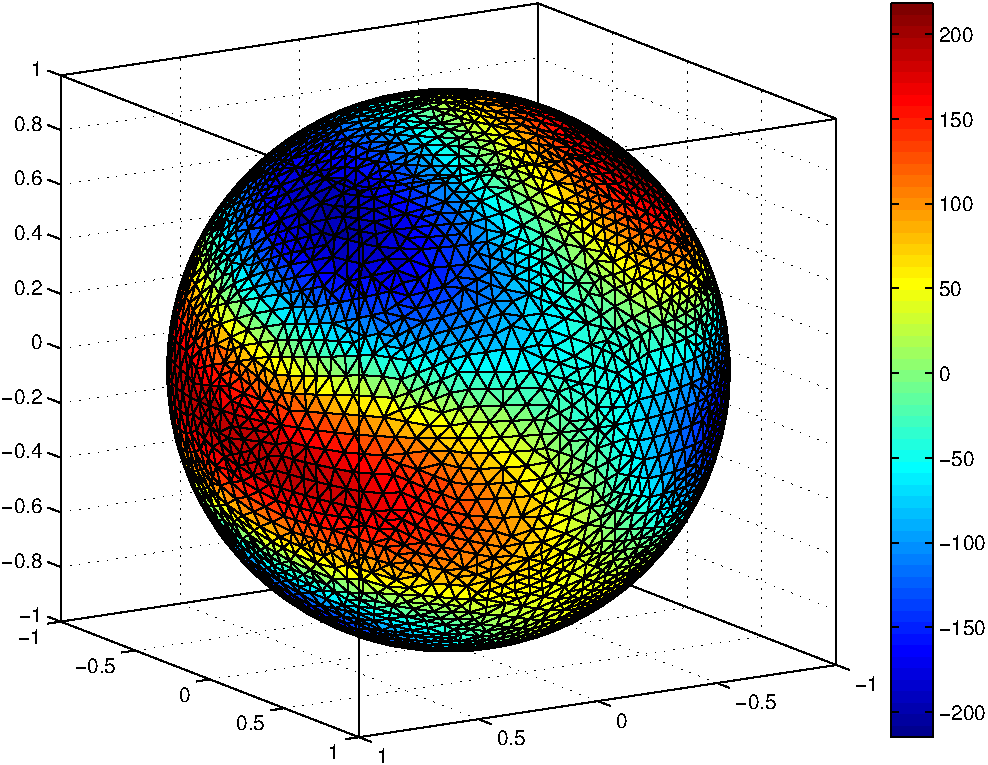
\includegraphics[width=\textwidth]{fig/sphere_mix_real.pdf}
% Komentář: Představím motivaci – závislostní stromy vznikající z textu mohou obsahovat opakující se vzory, které lze komprimovat.
\end{frame}

\begin{frame}{Cíle projektu}
\begin{itemize}
  \item Komprimovat syntaktické stromy
  \item Porovnat různé metody
  \item Vyhodnotit efektivitu
\end{itemize}
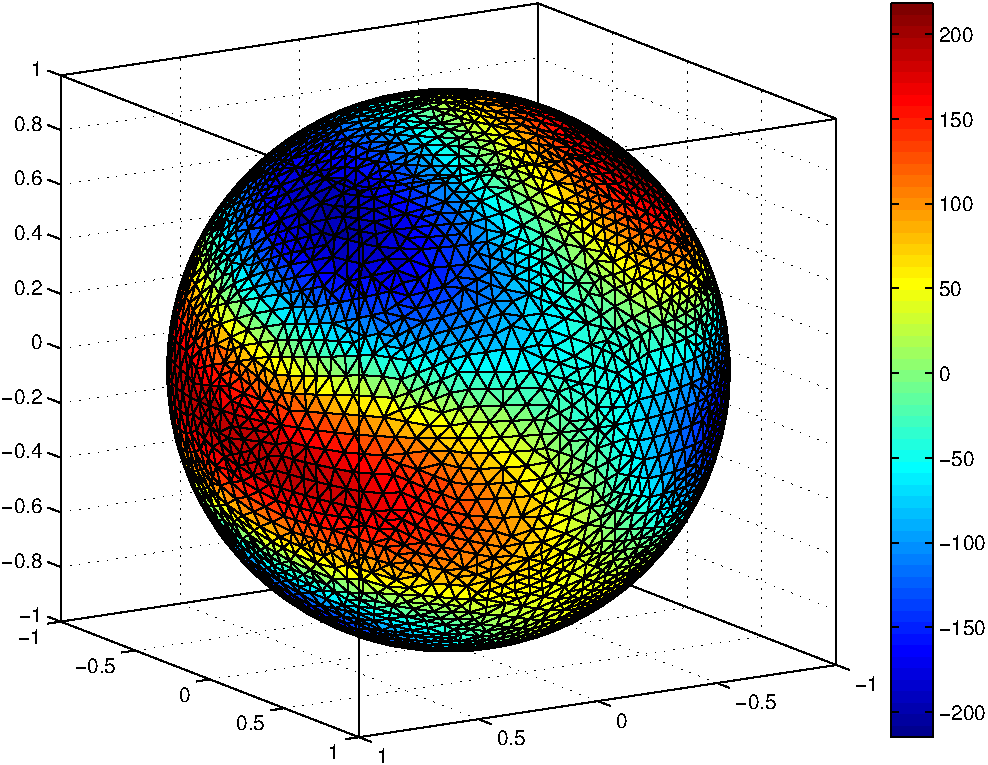
\includegraphics[width=0.8\textwidth]{fig/sphere_mix_real.pdf}
% Komentář: Stručně shrnu, že projekt má experimentální charakter – zkoumám různé strategie a jejich výkonnost.
\end{frame}

\section{Zpracování dat}
\begin{frame}{Z textu na strom}
\begin{itemize}
  \item MorphoDiTa → lemmatizace
  \item UDPipe → syntaktický strom
\end{itemize}
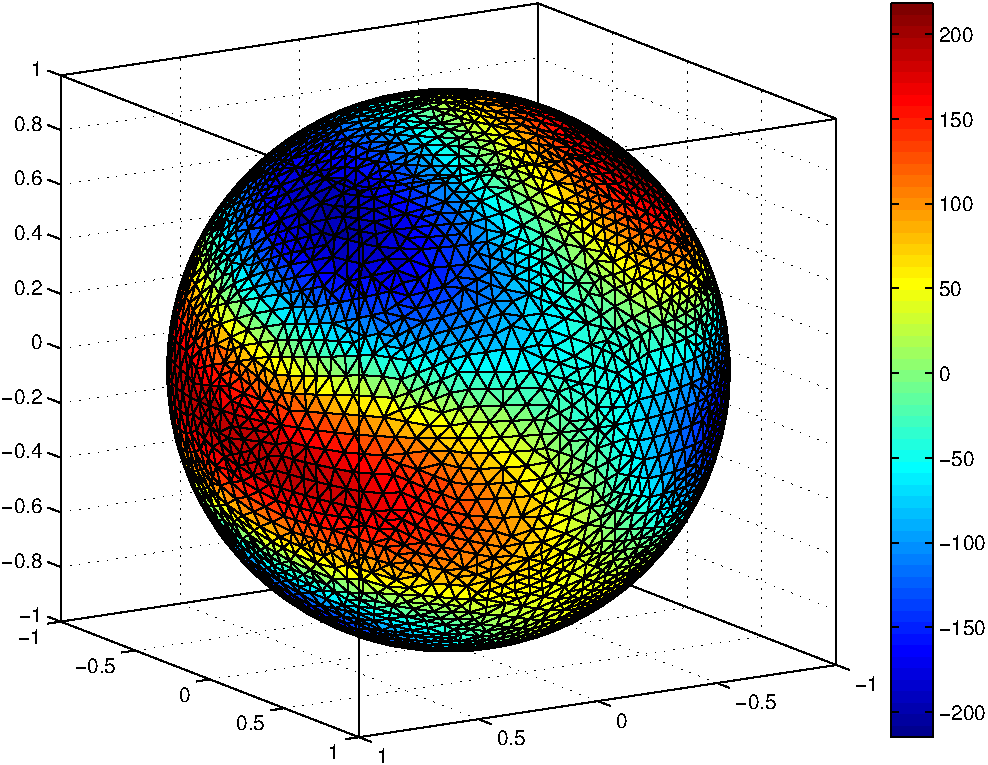
\includegraphics[width=\textwidth]{fig/sphere_mix_real.pdf}
% Komentář: Vysvětlím, jaké nástroje jsem použil a jak vypadá výstup - závislostní strom.
\end{frame}

\section{Architektura}
\begin{frame}{Struktura knihovny}
\begin{itemize}
  \item Vzor Pipes and Filters
  \item Moduly pro analýzu, kompresi, dekompresi
  \item Konzolová aplikace pro testování
\end{itemize}
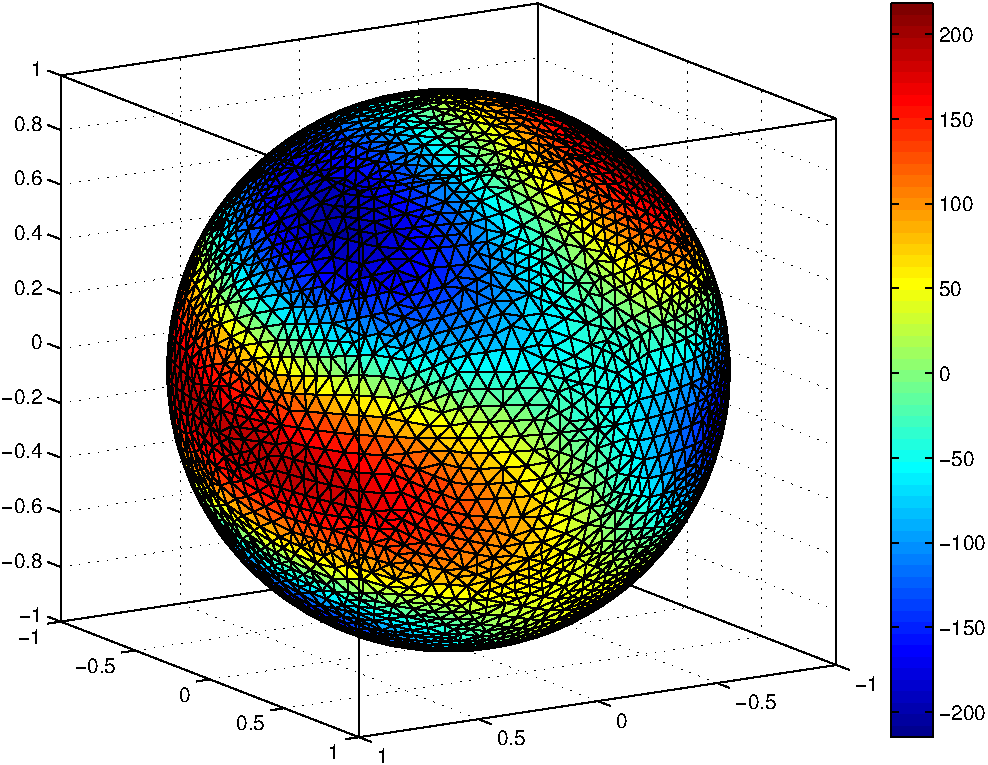
\includegraphics[width=0.9\textwidth]{fig/sphere_mix_real.pdf}
% Komentář: Předvedu, jak je knihovna navržená a že je flexibilní pro další experimenty.
\end{frame}

\begin{frame}{Pipeline scénáře}
\begin{itemize}
  \item Komprese: Text → Strom → Komprese
  \item Dekompres: Načtení → Dekomprese → Ověření
\end{itemize}
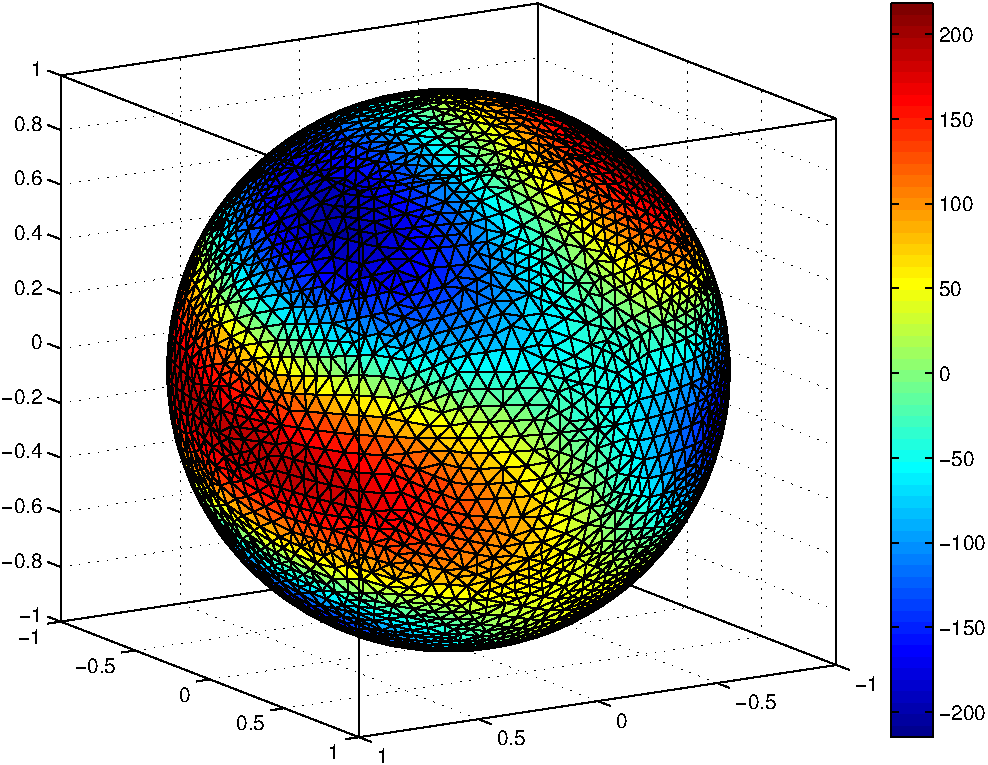
\includegraphics[width=0.9\textwidth]{fig/sphere_mix_real.pdf}
% Komentář: Ukážu příklad datového toku. Zdůrazním modulární návrh.
\end{frame}

\section{Algoritmy}
\begin{frame}{Algoritmus RePair}
\begin{itemize}
  \item Hledání opakujících se párů
  \item Nahrazení neterminály
  \item Vytvoření gramatiky
\end{itemize}
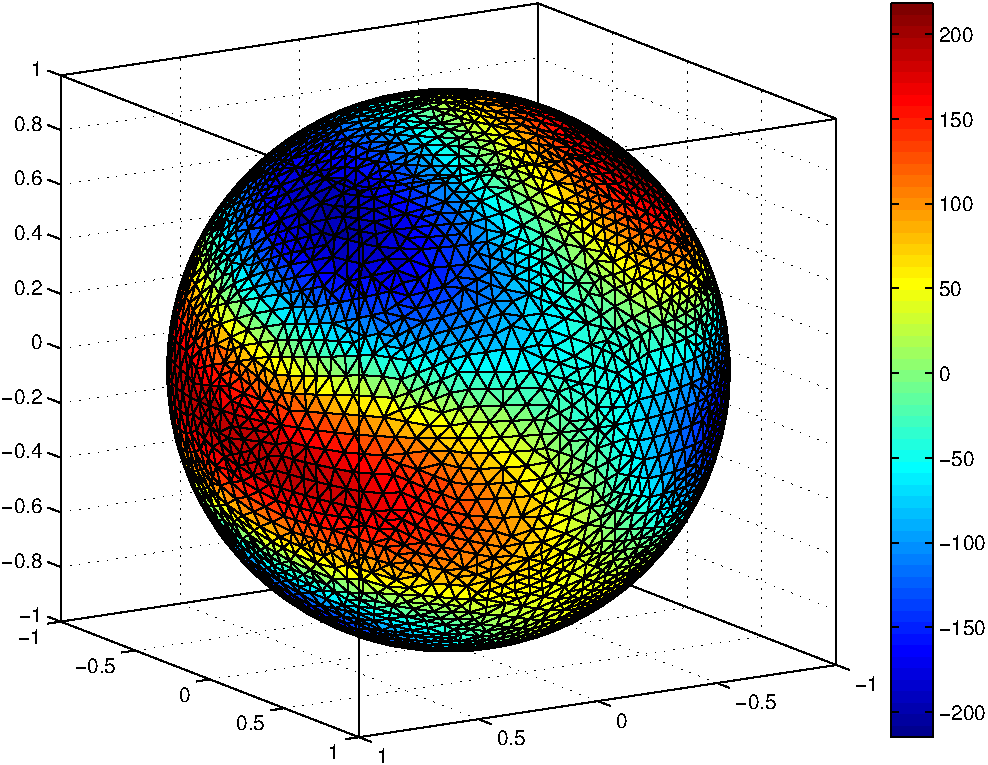
\includegraphics[width=\textwidth]{fig/sphere_mix_real.pdf}
% Komentář: Vysvětlím jednoduše princip RePair – hledáme opakující se sekvence a postupně je nahrazujeme.
\end{frame}

\begin{frame}{TreeRePair – bez linearizace}
\begin{itemize}
  \item Hledání opakujících se podstromů
  \item Hodnocení podle četnosti a velikosti
  \item Nahrazení pravidly
\end{itemize}
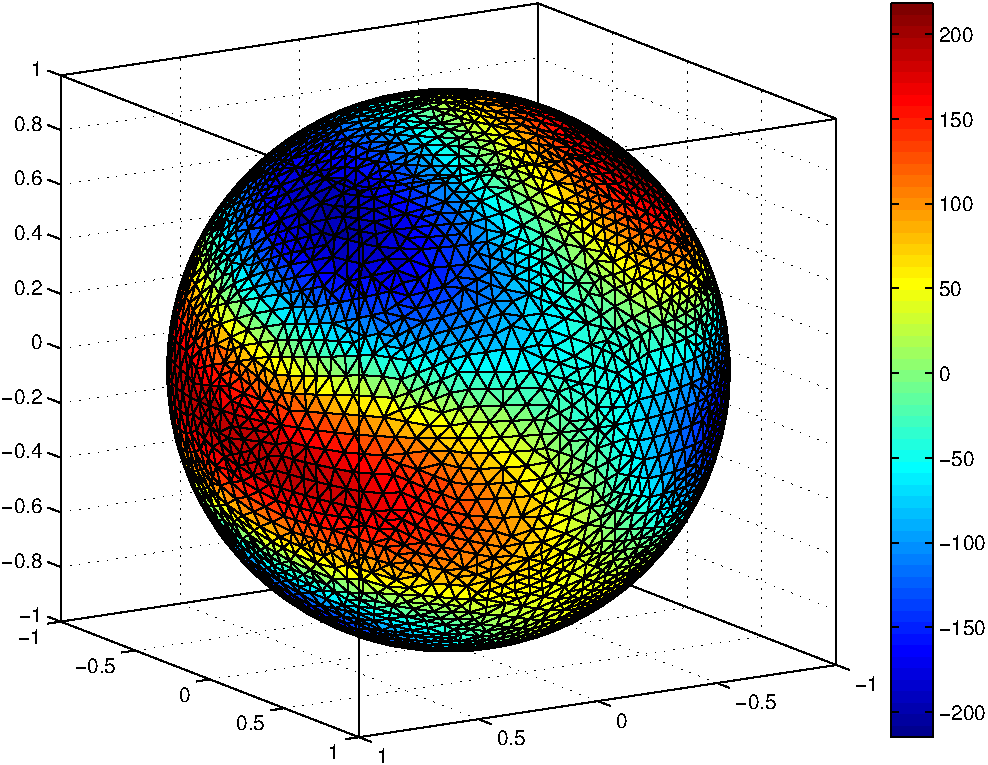
\includegraphics[width=\textwidth]{fig/sphere_mix_real.pdf}
% Komentář: Stromy se přímo zpracovávají – nehledáme sekvence, ale opakované části stromu.
\end{frame}

\begin{frame}{Linearizace + RePair}
\begin{itemize}
  \item Preorder průchod → sekvence
  \item RePair → pravidla
  \item Vylepšení: n-gramy, kontext
\end{itemize}
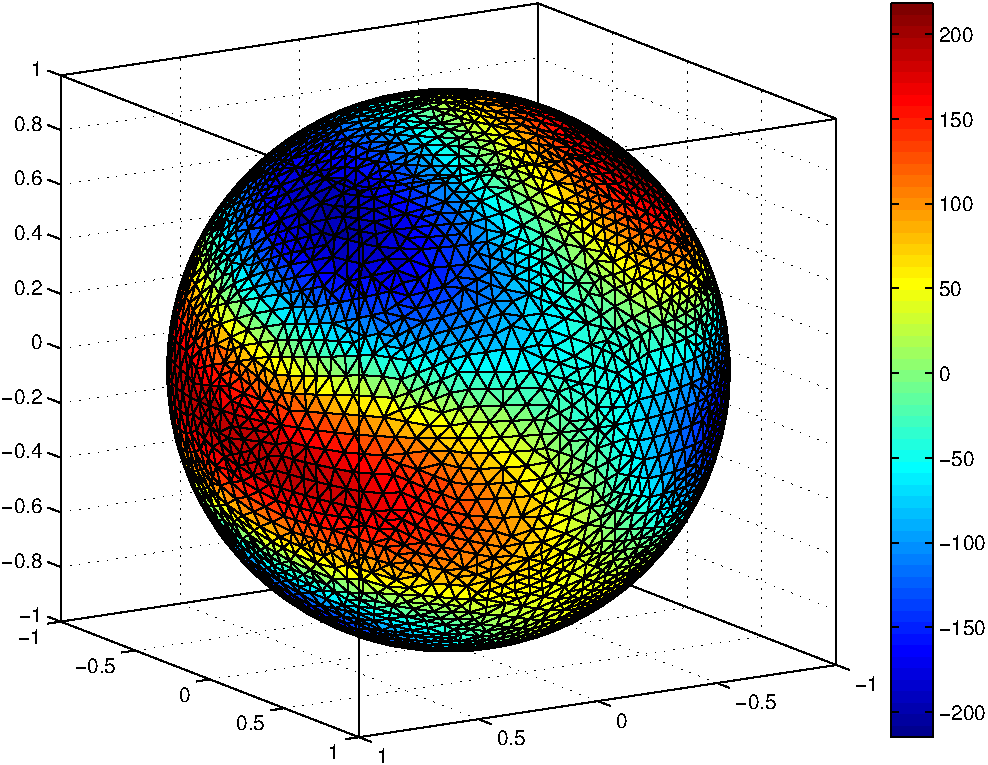
\includegraphics[width=\textwidth]{fig/sphere_mix_real.pdf}
% Komentář: Převedeme strom na text a použijeme RePair. Je to rychlejší, ale může ztratit část struktury.
\end{frame}

\section{Výsledky}
\begin{frame}{Shrnutí výsledků}
\begin{itemize}
  \item Linearizace + RePair: nejlepší průměrné výsledky
  \item TreeRePair: náročnější, méně efektivní
  \item Skutečná komprese: cca 9 % případů
\end{itemize}
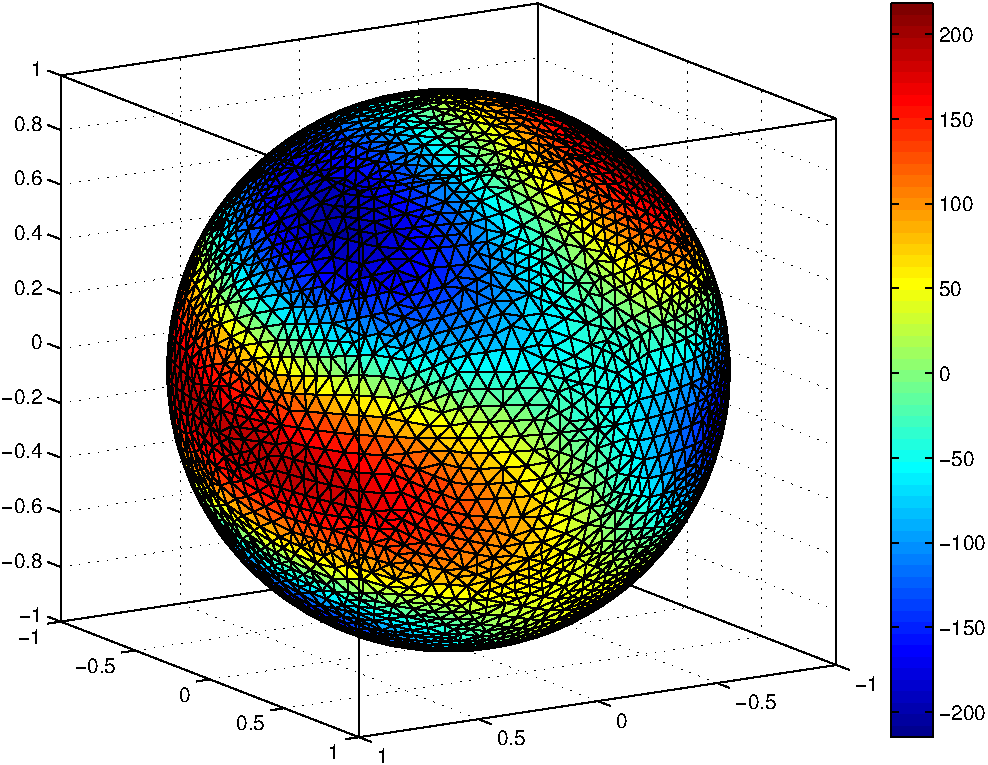
\includegraphics[width=0.9\textwidth]{fig/sphere_mix_real.pdf}
% Komentář: Zhodnotím výkonnost metod. Nejlepší poměry měla optimalizovaná linearizace + RePair.
\end{frame}

\begin{frame}{Závěr a výhled}
\begin{itemize}
  \item Komprese stromů není triviální
  \item Optimalizace výrazně pomáhají
  \item Možnosti do budoucna: paralelizace, adaptivní metody
\end{itemize}
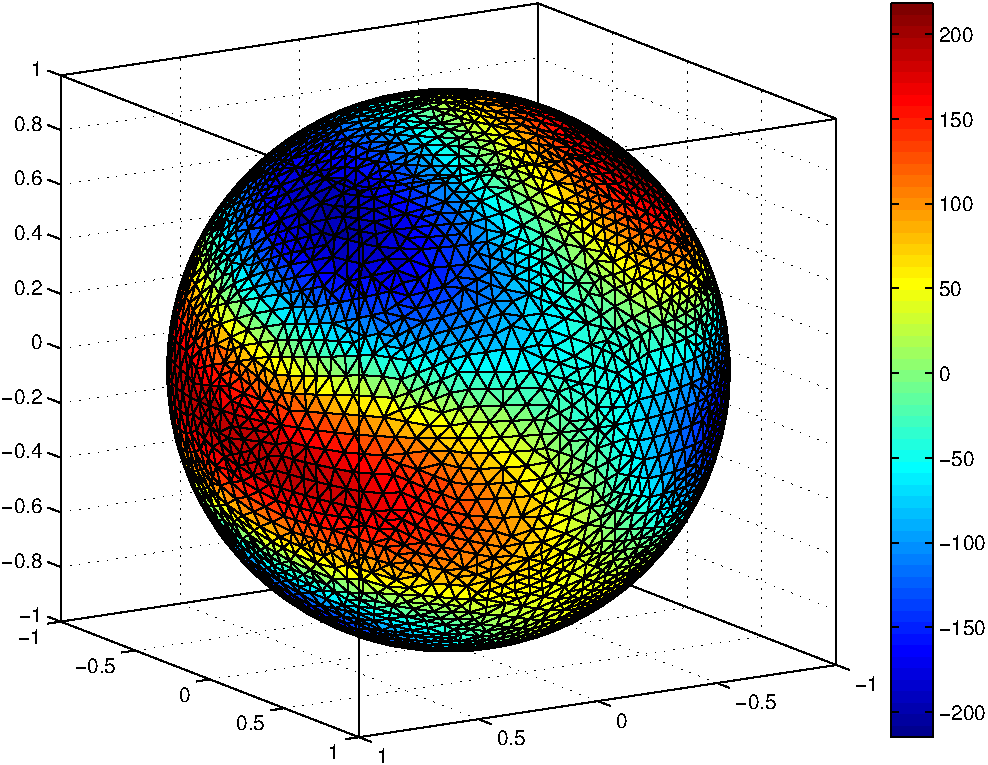
\includegraphics[width=0.8\textwidth]{fig/sphere_mix_real.pdf}
% Komentář: Shrnu zjištění – komprese má smysl, ale není jednoduchá. Budoucnost vidím v chytrém přepínání a kombinacích metod.
\end{frame}

\end{document}
